\section{Architektur}
Eine Architektur ist eine \textbf{Abstraktion} in welcher etwas zusammenfassend und vereinfacht dargestellt wird.

Mittels einer Architektur wird ein System beschrieben:

\begin{description}
	\item[Struktur und Aufbau] werden durch Elemente wie Sub- und Teilsystemen dargestellt.
	\item[Softwareteile] können mittels Aufgaben, Zuständigkeiten und Komponenten beschrieben werden.
	\item [Beziehungen] untereinander werden mit Abhängigkeiten, Schnittstellen und Datenflüsse modelliert.
\end{description}

\subsection{Aspekte der Architektur}
\begin{description}
	\item[Grundlegende Struktur] Schichten, Client/Server, n-tiers, Architekturmuster
	\item[Kommunikation und Verarbeitung] Kommunikationsmuster (Synchron/Asynchron), Verteilbarkeit, Parallelität, Performance, Robustheit
	\item[Technologien] Userinterface (Fat-, Rich- oder Thin-Client), Persistenz der Daten (Frameworks, O/R-Mapping), Referenzarchitekturen
	\item[Qualitätsaspekte] Wartungsfreundlichkeit, Erweiterbarkeit
\end{description}

\subsection{System und Subsystem}
''Das Gebilde, Zusamengestellte, Verbundene''. Ein System ist die Gesamtheit von Elementen, welche aufgaben-, sinn- oder zweckgebunden sind. Verfügt über klare Abgrenzung zu seiner Umwelt und wird organisiert durch Struktur und Beziehung.

\subsection{Softwaresysteme und Subsysteme}
Softwaresysteme werden wenn möglich immer zerlegt in einzelne Subsysteme (Teilsysteme). Zerlegung erfolgt meist mehrstufig hierarchisch. Subsysteme haben eine gewisse Unabhängigkeit und kommunizieren nur über wohldefinierte Schnittstellen miteinander. Dies ermöglicht folgende Vorteile:
\begin{itemize}
	\item präzisere Schätz- und Planbarkeit
	\item unabhängige Entwicklung möglich
	\item einfache Testbarkeit
	\item Potential für Wiederverwendung höher
	\item grössere Sicherheit
	\item höhere Stabilität und Robustheit
\end{itemize}
Diese Punkte sollten auch als Motivation gelten für eine gute Architektur. Es wird einfacher, verständlicher und übersichtlicher!

\subsection{Komponenten und (Sub-)systeme}
Eine Komponente ist eine softwaretechnische Einheit mit welcher man ein System realisieren kann. Ein System braucht nicht zwingend eine Komponente. Eine Komponenten kann zur Realisation von mehreren Systemen verwendet werden. Komponente und System sind orthogonal.


\subsection{Architekturmuster}
Beschreibt als Konzept den Grundaufbau eines ganzen Systems. Wohingegen Entwurfsmuster nur Konzepte für Teilprobleme sind. Architekturmuster sind nicht so stark vereinheitlicht wie Entwurfsmuster. Architekturmuster gibt es für verschiedene Aspekte: Um komplexe Systeme zU strukturieren, für verteilte Systeme, für interaktive Systeme, usw.

\subsubsection{Logische Aufteilung}
\paragraph{Schichten} Mittels Schichten kann ein System aufbauend, funktional und getrennt gegliedert werden. Die Kommunikation erfolgt über wohldefinierte Schnittstellen. Abhängigkeit nur in Richtung der tieferliegenden Schicht. Achtung: Bei physischer Verteilung der einzelnen Schichten spricht man von \textbf{tiers}.

\paragraph{Schichtenbildung} Nach folgenden Kriterien möglich: Logisch, Technologisch, Abstraktionsebene. Kann in Kombination hierarchisch verfeinert werden:
\begin{enumerate}
	\item Logische Schichtung
	\item Abstraktionslevel
	\item Technologie
\end{enumerate}
	
Beispiel mittels Java-Packages:
\textit{ch.domain.system.layerx, ch.domain.system.subsystem.layery}

\paragraph{Logische 3 Schichten-Architektur} Eine solche Aufteilung lohnt sich fast immer, unabhängig von der späteren physischen Verteilung.
\begin{description}
	\item[Präsentation] aka Presentation Layer, (G)UI-Layer. Visualisierung, User-Interface, UI-Logik. z.B. Bestellmaske für Artikel.
	\item[Geschäftslogik] aka Business(logic) Layer, Domain Layer. Implementation der Geschäftsprozesse und -modelle. z.B. Ablauf einer Bestellung, Modell eines Artikel.
	\item[Datenhaltung] aka Data Layer, Persistence Layer. Persistente Datenspeicherung, Datenlogik. z.B. Speicherung der Artikeldaten in einem RDBMS.
\end{description}

\paragraph{Verfeinerung Präsentationsschicht} Bei einem reinen Rich-GUI/Client ist es durchaus möglich, die reine Präsentation (Formulare, Dialoge) von der Präsentationslogik noch stärker zu trennen. Bspw. mittels MVC. Bei Thin-Clients (Web/HTML) ist die Trennung sogar zwingend notwendig. View wird durch HTML realisiert, Modelle und Präsentationslogik müssen im Server sein.

\paragraph{Verfeinerung Geschäftslogikschicht} Hier kann man weiteraufteilen in Business Objects bzw. Domain Objects. Dies ist ein reines objektorientiertes Modell, unabhängig von Präsentation als auch von Persistenz, enthalten Daten und Methoden. Zum Anderen kann man weiter aufteilen in Business Services. Enthält Klassen für die Geschäftsprozesse, arbeitet mit Business Objects. Bspw. ''Bestellen''. Kann technologisch noch weiter verfeinert werden. Einen Business Service als Webservice anbieten.

\paragraph{Verfeinerung Datenhaltungsschicht} Abstraktion der reinen Datenlogik. Diese ist unabhängig vom DBMS und vom physischen Datenmodell. Bspw. mittels O/R-Mapping. Transparentes Einbinden von Legacy-Systemen. Abstraktion mehrere Backend (DBMS)-Systeme.

\paragraph{Resultat dieser Verfeinerung}
Wenn man diese Verfeinerung vornimmt kommt man zu dieser 6-Schichten Architektur.
\begin{enumerate}
	\item Visualisation, User Interface: Formulare, Dialoge 
	\item User Interface Logik: Steuerung des UI, Ablauf
	\item Business Services, Business Logik: Fachliche Prozesse
	\item Business Objects, Business Modell: Fachliches Modell
	\item Datenlogik, Integrität: Fachliches Datenmodell
	\item Infrastruktur: z.B. O/R-Mapping-/Persistenzframework
\end{enumerate}
Bei mehr als 3 Schichten, spricht man in der Regeln von n-Schicht-Architektur.

\paragraph{Was ist die optimale Anzahl Schichten?}
Es gibt Vorteile:
\begin{itemize}
	\item Bessere Strukturierung, einzelne Schichten klarer und einfacher.
	\item Grössere Chance für Wiederverwendung
	\item Höhere Flexibilität z.B. Austausch einzelner Schichten
	\item Bessere Skalierbarkeit
	\item Einfachere und präzisere Planung/Schätzbarkeit
	\item Parallele und getrennte Entwicklung möglich.
\end{itemize}

.. und Nachteile:
\begin{itemize}
	\item Komplexität des gesamten Systems wird grösser
	\item Mehrere Schnittstellen, mehr Aufwand, mehr Planung.
\end{itemize}

\subsubsection{Physische Aufteilung}
\paragraph{Verteilte Architekturen: tiers} Schichtenbildung ist eine fundamentale Grundlage um verteilte Architekturen zu realisieren. Naheliegend eignen sich besonders die Schichtengrenzen zur Auftrennung um Teile auf verschiedene Systeme zu deployen. Wenn vorhandene Schichten auch physisch getrennt werden, spricht man von tiers. Populäre verteilte Architekturen sind: Client/Server (2-tier), Web-Anwendung (n-tier).

\paragraph{2-tier: Client/Server}
Klassisch: GUI-Client greift direkt auf DB-Server zu. Typisch kennt man n-Clients und 1-DB Server (n:1). Natürlich auch n:n möglich. Dies kennt man heute eher im firmeninternen Bereich (Intranet). Ist häufig auch plattformspezifisch. Die Datenhaltung und Integrität wird mittels Datenmodell und Constraints gewährleistet, die Datenlogik wird u.a. mittels Trigger/Procedures realisiert.

Es ist eine einfache Architektur und gut überblickbar. Die Datenhaltung ist zentral. Jedoch für grosse / komplexe Anwendungen gibt es keinen guten Ort für die Business-Logik. Der Client wird fat, Bussiness-Logik ist redundanten vorhanden, Änderungen verlangen vollständiges redeployment. Falls im DB-Server programmiert wird, dann gibt es x unterschiedlche Sprachen je nach DMS-Hersteller. Hohe Last durch Prozeduren, Triggers und co. Wenn man einen Teil im Client und einem Teil im DB Server implementiert, dann ist es oft schwierig zu sagen, was nun wo hin soll. Demzufolge auch schlechte Wartbarkeit, weniger elegant.

\paragraph{3-tier Architektur}
Basis für die meisten Enterprise Architekturen. Typisch m:1:n (Client:Business-Daten).

Keine Redundanz der Logik vorhanden. Potential: Einbinden mehrere verschiedener Datenquellen. Verschiedene Clients realisierbar (Technologie, Umfang, Fachlich). Echte Zentralisierung von reiner Business-Logik möglich. Clients können ''rich'' sein, sind aber nicht ''fat''.

Die Aufteilung ermöglicht einen effizientere Nutzung der vorhandenen Rechenleistung. Bzw. Clients können redimensioniert werden. Falls das Design aber schlecht ist, dann kann die Kommunikation zwischen den verteilten Tiers kritisch werden. Potentiell hoher Ressourcenbedarf (Speicher) im Middle-Tier.

\subsection{MVC}
Dies ist ein Designmuster mit dem Ziel Datemodell von seiner Darstellung und deren Steuerung strikte zu trennen. Wichtig: Die exakte Implementation variiert nach Anwendungsfall und Programmiersprache!

\paragraph{Anwendungsfall 1: MVC in GUI-Widgets wie Swing} Controller und View sind oft zusammengefasst. Das Model existiert jedoch autonom.

\paragraph{Anwendungsfall 2: MVC auf Applikationsebene} Model ist meist eine ganz normale Java-Klasse. Mehrere Views können die Daten darstellen. Änderungen im Modell werden an die Views gesendet. Modell darf aber View nicht kennen (Observer)! Ein Controller verändert die Modelle und ordnet den Views die entsprechenden Modelle zu. Bsp: Modell einer Kundenadresse. Zwei Views: Detailliertes Formulare und als Zeile in Tabellenansicht.

\begin{figure}[h!]
\centering
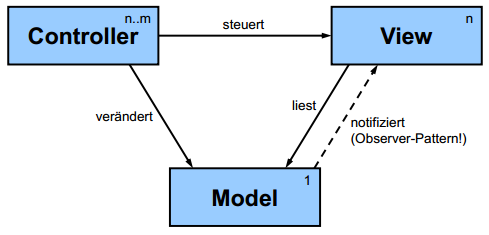
\includegraphics[width=0.7\linewidth]{fig/mvc}
\caption{MVC}
\label{fig:mvc}
\end{figure}

\paragraph{Implementationsvarianten} Kopplung zwischen Model und View. Observerpattern zwischen Modell und View oder über Controller. Statisches Modell: Notifikation über Änderungen im Modell (eher bei grösseren Modellen mit wenig Änderungen). Dynamisches Modell: Aktuelles Modell wird der View regelmässig übergeben (eher bei kleineren Modellen mit vielen Änderungen).

\paragraph{MVC in Webapplikationen} MVC Architektur ist bedingt durch die Technologie von Web-Applikationen eine Herauserforderung. Es besteht oft die Gefahr View und Business-Logic zu vermischen. Modell kann jeweils relativ einfach extrahiert werden. Im Laufe der Zeit sind zwei MVC-Varianten entstanden:

\begin{figure}[h!]
\centering
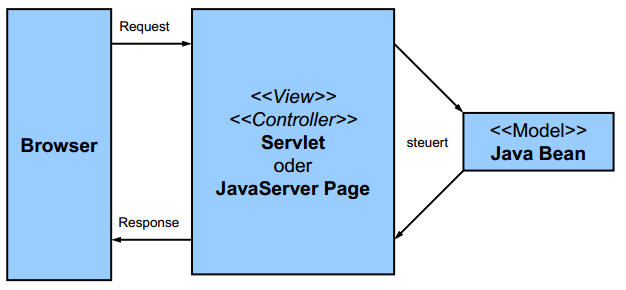
\includegraphics[width=0.7\linewidth]{fig/mvc-web-1}
\caption{MVC Variante 1: Alt und eher schlecht. (View Controller vermischt)}
\label{fig:mvc-web-1}
\end{figure}

\begin{figure}[h!]
\centering
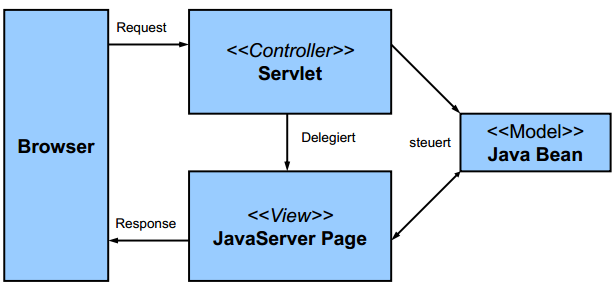
\includegraphics[width=0.7\linewidth]{fig/mvc-web-2}
\caption{MVC Variante 2: Neu und eher besser.}
\label{fig:mvc-web-2}
\end{figure}



\subsection{Diskussion: Thin-, Richt-, Fat-Client}
Ein Thin-Client enthält nur die Präsentationsschicht. Eine HTML-Seite ist quasi ein Thin-Clien.t
Der Rich-Client ist beispielsweise ein Java-Programm, welcher aber in einer n-Tier Architektur steckt. Auf dem Client ist nur die Präsentation geregelt. Die Business-Logik befindet sich auf einem andern tier. Der Fat-Client ist die Variante einer 2-Tier-Architektur. Business Logik steckt im Client.
